\chapter{Case study overview}

To compare the frameworks, a simple chatbot will be designed and created employing the techniques above. The chatbot will be a food ordering chatbot that offers the user a menu and takes in orders, similar to Domino's bot.

\section{Conversational state diagram}

To shape the bot, a conversational diagram needs to be created first. This diagram explains the main flow of the conversation, and the steps to reach the eventual purpose of the bot. In this case ordering food.

\begin{figure}[p]
	\centering
	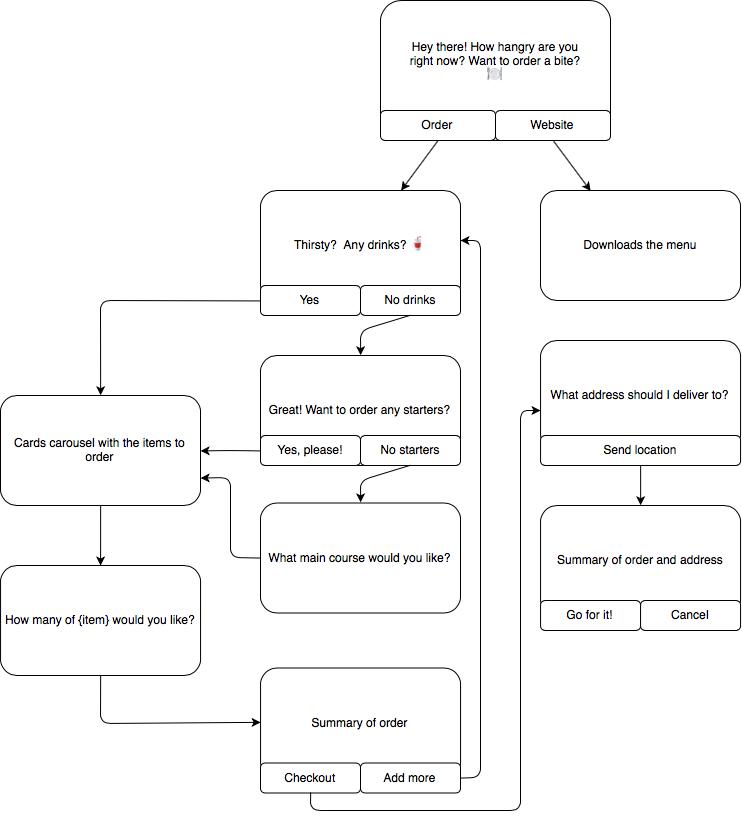
\includegraphics[width=\textwidth]{conversationalflow}\label{fig:conversationalflow}
	\caption{Conversational flow diagram for the food ordering bot~}
\end{figure}
